\chapter{Deeplearning}
Le principali tipologie di apprendimento sono:
\begin{itemize}
    \item \textbf{Supervisionato} (Supervised): i dati utilizzati per l'apprendimento
          sono etichettati (label).
    \item \textbf{Non supervisionato} (Unsupervised): i dati utilizzati per
          l'apprendimento non sono etichettati.
\end{itemize}
Inizialmente, le architetture di deeplearning sono state composte da particolari
strutture simili agli enconder-decoder chiamate \textbf{autoencoder}. Queste
strutture sono reti neurali, costruite con una particolare struttura a clessidera,
il cui compito è quello di imparare come ricostruire l'input.
\begin{figure}[!ht]
    \centering
    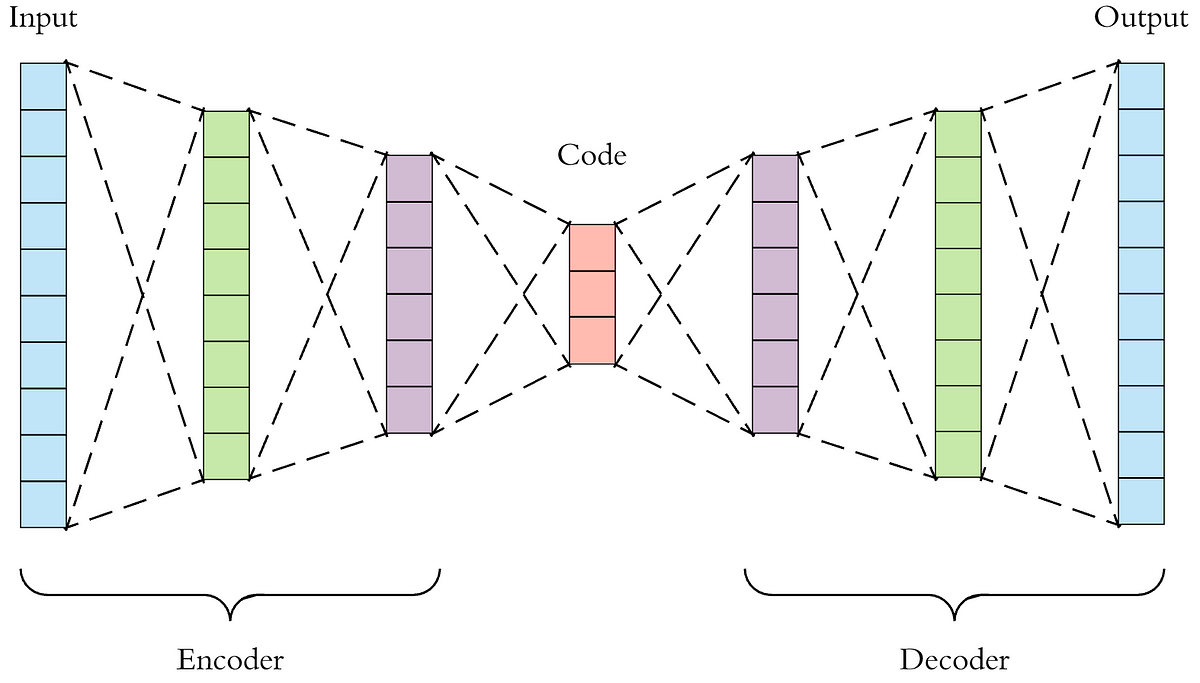
\includegraphics[scale=0.5]{img/reti/autoencoder.png}
    \caption{Autoencoder}
    \label{fig:autoencoder}
\end{figure}
La metodologia di apprendimento utilizzata da questa rete prende il nome di
\textbf{fake task}, ovvero si adotta una metodologia supervisionata in cui non si
ha una label, ma quello che si vuole ottenere è l'input stesso. L'obiettivo
è ridurre l'errore sulla ricostruzione dell'input. Il loro risultato è dovuto
alla loro struttura a collo di bottiglia che separa la rete in due:
\begin{itemize}
    \item \textbf{Enconder}: impara a codificare l'input utilizzando poche
          informazioni (funzione di codifica).
    \item \textbf{Denconder}: impara a decodificare l'input partendo da poche
          informazioni (funzione di decodifica).
\end{itemize}
L'algortimo di apprendimento di queste reti spesso è una delle tante implementazioni
di backpropagation, applicandolo su ciascun neurone di uscita.

Per gli autoencoder si deve obbligatoriamente avere sempre una struttura a clessidra
con la strozzatura centrale, la quale permette di generare la codifica e separare
le due reti. In aggiunta, l'architettura non prevede che ci siano collegamenti
tra encoder e decoder altrimenti la codifica nella strozzatura non è più consistente.

Le architetture odierne di deeplearning si basano su strutture neurali e utilizzano i
\textbf{tranformer}, componenti neurali che prendono in input sia il nuovo input,
sia un vecchio output del trasformer. Sono componenti fondamentali per la generazione
di informazioni. L'apprendimento di queste reti si basa su strutture \textbf{feed-forward}
e su componenti \textbf{Attention}, quest'ultimi fondamentali perché permettono
l'effettivo cambiamento dei valori.
\begin{figure}[!ht]
    \centering
    \includegraphics[scale=0.5]{img/deepl/tranformer.png}
    \caption{Struttura di un transformer}
    \label{fig:attention}
\end{figure}
Prima di arrivare ai transformer si è passati dagli autoencoder, a \textbf{Word2Vec},
un modello neurale utilizzato per problemi di \textbf{NPL}. Più precisamente si occupa
di associare per ogni parola del linguaggio un vettore di numeri reali, in questo
modo è possibile rappresentare le singole parole in uno spazio $n$-dimensionale.
Questa proprietà ha permesso di scoprire una proprietà: parole simili vengono
rappresentate in una regione vicina dello spazio. Questo è dato dal fatto che
le reti vengono allenate su tutti i testi raggiungibili e l'assegnamento del vettore
si effettua in base a quante volte due parole vengono veste vicine in una frase.
Quindi la rete riesce a codificare come vettori simili parole simili, infatti c'è
una corrispodenza geometrica col significato.

Successivamente si è passati ai \textbf{denoising autoencoder}, ovvero rimozione
del rumore e ricostruzione dell'input originale. Queste reti vengono allenate dando
in input il dato sporcato in precedenza, successivamente l'output viene confrontato
con l'input originale.

In seguito, sono stati introdotti i componenti \textbf{Attention}, composti da 3
elementi in input e il suo compito è di assegnare in automatico diversi pesi
agli elementi in input. Queste reti permettono quindi di cambiare i pesi degli input
portando a dei vantaggi notevoli, per esempio, si possono interpretare parole ambigue
in base al contesto.

Infine, si è passati ai tranformer, introcendo la ricorrenza dei dati in modo da
considerare in input i vecchi dati della rete, sfasati, con un meccanismo di
Attention.

I modelli di deeplearning vengono allenati in 2 fasi:
\begin{itemize}
    \item \textbf{pretraining generico}: allenamento non supervisionato, si allena
          la rete in modo generale senza specificare un particolare task. Questa
          fase è la più pesante e permette di definire un primo stato di partenza
          dei parametri.
    \item \textbf{finetuning}: si prende la rete preallenata e si addestra per un
          task specifico utilizzando la metodologia supervisionata.
\end{itemize}
In questo modo è possibile ridurre i tempi di addestramento e rendere riutilizzabile
la stessa rete per task simili.

Alla fine si arriva alla creazione di reti più complesse come GPT, basata sempre
su trasformer e attention, ma addestrata in 2 fasi, con la possibilità di effettuare
del reinforcement learning per migliorare ancora di più i risultati.